\documentclass[xetex,mathserif,serif]{beamer}
\usepackage{polyglossia}
\setdefaultlanguage[babelshorthands=true]{russian}
\usepackage{minted}
\usepackage{tabu}

\useoutertheme{infolines}

\usepackage{fontspec}
\setmainfont{FreeSans}
\newfontfamily{\russianfonttt}{FreeSans}

\setbeamertemplate{blocks}[rounded][shadow=false]

\setbeamercolor*{block title alerted}{fg=red!50!black,bg=red!20}
\setbeamercolor*{block body alerted}{fg=black,bg=red!10}

\tabulinesep=1.2mm

\title{Язык F\#}
\subtitle{Введение}
\author{Юрий Литвинов}
\date{23.11.2017}

\begin{document}
	
	\frame{\titlepage}

	\section{Введение}

	\begin{frame}
		\frametitle{F\#}
		\begin{itemize}
			\item Типизированный функциональный язык для платформы .NET
			\item НЕ чисто функциональный (можно императивный стиль и ООП)
			\item Первый раз представлен публике в 2005 г.
			\item Создавался под влиянием OCaml (практически диалект OCaml под .NET)
			\item Использует .NET CLI
			\item Компилируемый и интерпретируемый
			\item Используется в промышленности, в отличие от многих чисто функциональных языков
		\end{itemize}
	\end{frame}

	\begin{frame}
		\frametitle{Что скачать и поставить}
		\begin{itemize}
			\item Под Windows --- Visual Studio, из коробки
			\item Под Linux
			\begin{itemize}
				\item Mono + MonoDevelop + F\# Language Binding, из репозиториев
				\item .NET Core + Visual Studio Code
			\end{itemize}
			\item Прямо в браузере: http://www.tryfsharp.org/Learn
		\end{itemize}
	\end{frame}
	
	\begin{frame}[fragile]
		\frametitle{Пример программы}
		\begin{minted}{fsharp}
printfn "%s" "Hello, world"
		\end{minted}
		Сравните с
		\begin{minted}{csharp}
namespace HelloWorld
{
    class Program
    {
        static void Main(string[] args)
        {
            System.Console.WriteLine("Hello, world!");
        }
    }
}
		\end{minted}
\end{frame}

	\begin{frame}[fragile]
		\frametitle{Ещё пример}
		\begin{minted}{fsharp}
let rec factorial x =
    if x = 1 then 1 else x * factorial (x - 1)
		\end{minted}
\end{frame}
	
	\section{Let-определения}

	\begin{frame}[fragile]
		\frametitle{let-определение}
		\begin{minted}{fsharp}
let x = 1
let x = 2
printfn "%d" x
		\end{minted}
		можно читать как
		\begin{minted}{fsharp}
let x = 1 in let x = 2 in printfn "%d" x
		\end{minted}
		и понимать как подстановку $\lambda$-терма
\end{frame}
		
	\begin{frame}[fragile]
		\frametitle{let-определение, функции}
		\begin{minted}{fsharp}
let powerOfFour x = 
    let xSquared = x * x
    xSquared * xSquared
		\end{minted}
		\begin{itemize}
			\item Позиционный синтаксис
			\begin{itemize}
				\item Отступы строго пробелами
				\item Не надо ";"
			\end{itemize}
			\item Нет особых синтаксических различий между переменной и функцией
			\item Не надо писать типы
			\item Не надо писать \textit{return}
		\end{itemize}
\end{frame}

	\begin{frame}[fragile]
		\frametitle{Вложенные let-определения}
		\begin{minted}{fsharp}
let powerOfFourPlusTwoTimesSix n =
    let n3 =
        let n1 = n * n
        let n2 = n1 * n1
        n2 + 2
    let n4 = n3 * 6
    n4
		\end{minted}
		\begin{itemize}
			\item \textit{n3} --- не функция!
			\item Компилятор отличает значения и функции по наличию аргументов
			\item Значение вычисляется, когда до \textit{let} <<доходит управление>>, 
					функция --- когда её вызовут. Хотя, конечно, функция --- тоже значение.
		\end{itemize}
\end{frame}

	\section{Типы}

	\begin{frame}[fragile]
		\frametitle{Типы}
		\begin{minted}{fsharp}
let rec f x =
    if x = 1 then 
        1 
    else 
        x * f (x - 1)
		\end{minted}

		\begin{alertblock}{F\# Interactive}
			\begin{minted}{fsharp}
val f : x:int -> int
			\end{minted}
		\end{alertblock}
		Каждое значение имеет тип, известный во время компиляции
\end{frame}

	\begin{frame}
		\frametitle{Элементарные типы}
		\begin{itemize}
			\item \textit{int}
			\item \textit{double}
			\item \textit{bool}
			\item \textit{string}
			\item ... (.NET)
			\item \textit{unit} --- тип из одного значения, (). Аналог void.
		\end{itemize}
	\end{frame}
	
	\begin{frame}[fragile]
		\frametitle{Кортежи (tuples)}
		\begin{minted}{fsharp}
let site1 = ("scholar.google.com", 10)
let site2 = ("citeseerx.ist.psu.edu", 5)
let site3 = ("scopus.com", 4)
let sites = (site1, site2, site3)

let url, relevance = site1
let site1, site2, site3 = sites
		\end{minted}
\end{frame}

	\begin{frame}[fragile]
		\frametitle{Value Tuples}
		\begin{minted}{fsharp}
let origin = struct (0,0)

let displace 
        ((x, y): struct (int * int))
        ((dx, dy): struct (int * int)) 
    =
    struct (x + dx, y + dy)
		\end{minted}
\end{frame}

	\begin{frame}[fragile]
		\frametitle{Лямбды}
		\begin{minted}{fsharp}
let primes = [2; 3; 5; 7]
let primeCubes = List.map (fun n -> n * n * n) primes
		\end{minted}
		\begin{alertblock}{F\# Interactive}
			\begin{minted}{fsharp}
> primeCubes;;
val it : int list = [8; 27; 125; 343]
			\end{minted}
		\end{alertblock}
		\begin{minted}{fsharp}
let f = fun x -> x * x
let n = f 4
		\end{minted}
\end{frame}

	\begin{frame}
		\frametitle{Списки}
		\begin{small}
			\begin{tabu} {| X[0.9 l p] | X[1 l p] | X[1 l p] |}
				\tabucline-
				Синтаксис                               & Описание                  & Пример                             \\
				\tabucline-
				\everyrow{\tabucline-}
				$[]$                                    & Пустой список             & $[]$                               \\
				$[expr; ...; expr]$                     & Список с элементами       & $[1; 2; 3]$                        \\
				$expr :: list$                          & cons, добавление в голову & $1 :: [2; 3]$                      \\
				$[expr\ ..\ expr]$                      & Промежуток целых чисел    & $[1 .. 10]$                        \\
				$[for\ x\ in\ list\ \rightarrow\ expr]$ & Генерированный список     & $[for\ x\ in\ 1..99\ \rightarrow\ x\ *\ x]$ \\
				$list\ @\ list$                         & Конкатенация              & $[1; 2]\ @\ [3; 4]$                \\
			\end{tabu}
		\end{small}
	\end{frame}

	\begin{frame}[fragile]
		\frametitle{Примеры работы со списками}
		\begin{minted}{fsharp}
let oddPrimes = [3; 5; 7; 11]
let morePrimes = [13; 17]
let primes = 2 :: (oddPrimes @ morePrimes)
		\end{minted}
		\begin{minted}{fsharp}
let printFirst primes =
    match primes with
    | h :: t -> printfn "First prime in the list is %d" h
    | [] -> printfn "No primes found in the list"			
		\end{minted}
\end{frame}

	\begin{frame}[fragile]
		\frametitle{Устройство списков}
		\begin{center}
			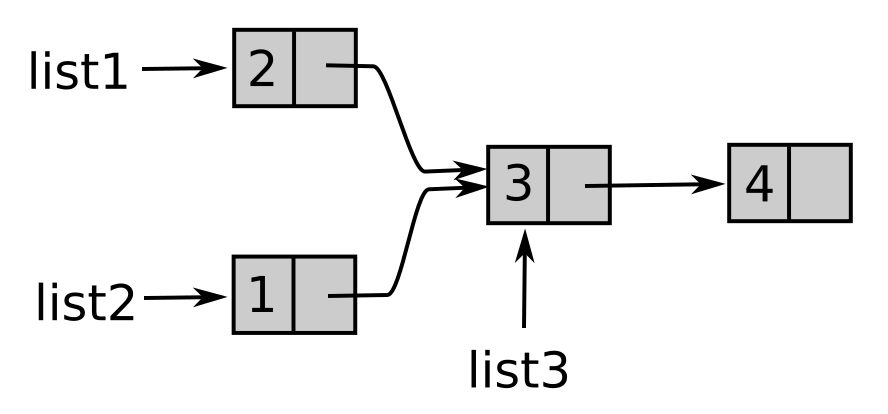
\includegraphics[width=0.4\textwidth]{lists.png}
		\end{center}
		\begin{minted}{fsharp}
let list3 = [3; 4]
let list1 = 2 :: list3
let list2 = 1 :: list3
		\end{minted}
		\begin{itemize}
			\item Списки немутабельны
			\item Cons-ячейки, указывающие друг на друга
			\item cons за константное время, @ --- за линейное
		\end{itemize}
\end{frame}

	\begin{frame}
		\frametitle{Операции над списками}
		\framesubtitle{Модуль Microsoft.FSharp.Collections.List}
		\begin{scriptsize}
			\begin{tabu} {| X[0.5 l p] | X[1 l p] | X[1 l p] | X[0.5 l p] |}
				\tabucline-
				Функция                & Описание                            & Пример                                              & Результат            \\
				\tabucline-
				\everyrow{\tabucline-}
				List.length            & Длина списка                        & $List.length\ [1;2;3]$                              & $3$                  \\
				List.nth               & n-ый элемент списка                 & $List.nth\ [1; 2; 3]\ 1$                            & $2$                  \\
				List.init              & Генерирует список                   & $List.init\ 3 (fun\ i\ \rightarrow\ i * i)$         & $[0; 1; 4]$          \\
				List.head              & Голова списка                       & $List.head\ [1; 2; 3]$                              & $1$                  \\
				List.tail              & Хвост списка                        & $List.tail\ [1; 2; 3]$                              & $[2; 3]$             \\
				List.map               & Применяет функцию ко всем элементам & $List.map\ (fun\ i\ \rightarrow\ i * i)\ [1; 2; 3]$ & $[1; 4; 9]$          \\
				List.filter            & Отбирает нужные элементы            & $List.filter\ (fun\ x\ \rightarrow\ x\ \%\ 2 <> 0)\ [1; 2; 3]$ & $[1; 3]$  \\
				List.fold              & "Свёртка"  & $List.fold\ (fun\ x\ acc\ \rightarrow\ acc * x)\ 1\ [1; 2; 3]$               & $6$                  \\
				List.zip               & Делает из двух списков список пар   & $List.zip\ [1; 2]\ [3; 4]$                          & $[(1, 3); (2, 4)]$   \\
			\end{tabu}
		\end{scriptsize}
	\end{frame}
	
	\begin{frame}[fragile]
		\frametitle{Тип Option}
		Либо \textit{Some что-то}, либо \textit{None}, представляет возможное отсутствие значения.
		\begin{minted}{fsharp}
let people = [ ("Adam", None); ("Eve" , None);
    ("Cain", Some("Adam","Eve"));
    ("Abel", Some("Adam","Eve")) ]
		\end{minted}
		\begin{minted}{fsharp}
let showParents (name, parents) =
    match parents with
    | Some(dad, mum) -> 
        printfn "%s, father %s, mother %s" name dad mum
    | None -> printfn "%s has no parents!" name
		\end{minted}
\end{frame}

	\section{Функции}

	\begin{frame}[fragile]
		\frametitle{Рекурсия}
		\begin{minted}{fsharp}
let rec length l =
    match l with
    | [] -> 0
    | h :: t -> 1 + length t

let rec even n = (n = 0u) || odd(n - 1u)
and odd n = (n <> 0u) && even(n - 1u)
		\end{minted}
\end{frame}

	\begin{frame}[fragile]
		\frametitle{Оператор $|>$}
		\framesubtitle{Pipe forward}
		\begin{minted}{fsharp}
let (|>) x f = f x
		\end{minted}

		\begin{minted}{fsharp}
let sumFirst3 ls = ls |> Seq.take 3 |> Seq.fold (+) 0
		\end{minted}
		вместо
		\begin{minted}{fsharp}
let sumFirst3 ls= Seq.fold (+) 0 (Seq.take 3 ls)
		\end{minted}
\end{frame}

	\begin{frame}[fragile]
		\frametitle{Оператор $>>$}
		\framesubtitle{Композиция}
		\begin{minted}{fsharp}
let (>>) f g x = g (f x)
		\end{minted}
		\begin{minted}{fsharp}
let sumFirst3 = Seq.take 3 >> Seq.fold (+) 0
let result = sumFirst3 [1; 2; 3; 4; 5]
		\end{minted}
\end{frame}

	\begin{frame}[fragile]
		\frametitle{Операторы $<|$ и $<<$}
		\framesubtitle{Pipe-backward и обратная композиция}
		\begin{minted}{fsharp}
let (<|) f x = f x
let (<<) f g x = f (g x)
		\end{minted}
		Зачем? Чтобы не ставить скобки:
		\begin{minted}{fsharp}
printfn "Result = " <| factorial 5
		\end{minted}
\end{frame}

	\begin{frame}[fragile]
		\frametitle{Каррирование, частичное применение}
		\begin{minted}{fsharp}
let shift (dx, dy) (px, py) = (px + dx, py + dy)
let shiftRight = shift (1, 0)
let shiftUp = shift (0, 1)
let shiftLeft = shift (-1, 0)
let shiftDown = shift (0, -1)
		\end{minted}
		\begin{alertblock}{F\# Interactive}
			\begin{minted}{fsharp}
> shiftDown (1, 1);;
val it : int * int = (1, 0)
			\end{minted}
		\end{alertblock}
\end{frame}

	\section{Сопоставление шаблонов}
	
	\begin{frame}[fragile]
		\frametitle{Сопоставление шаблонов}
		\begin{minted}{fsharp}
let urlFilter url agent =
    match (url, agent) with
    | "http://www.google.com", 99 -> true
    | "http://www.yandex.ru" , _ -> false
    | _, 86 -> true
    | _ -> false
		\end{minted}

		\begin{minted}{fsharp}
let sign x =
    match x with
    | _ when x < 0 -> -1
    | _ when x > 0 -> 1
    | _ -> 0
		\end{minted}
\end{frame}

	\begin{frame}[fragile]
		\frametitle{F\# --- не Prolog}
		Не получится писать так:
		\begin{minted}{fsharp}
let isSame pair =
    match pair with
    | (a, a) -> true
    | _ -> false
		\end{minted}
		Нужно так:
		\begin{minted}{fsharp}
let isSame pair =
    match pair with
    | (a, b) when a = b -> true
    | _ -> false
		\end{minted}
\end{frame}

	\begin{frame}
		\frametitle{Какие шаблоны бывают}
		\begin{small}
			\begin{tabu} {| X[0.9 l p] | X[1 l p] | X[1 l p] |}
				\tabucline-
				Синтаксис                               & Описание                  & Пример                  \\
				\tabucline-
				\everyrow{\tabucline-}
				$(pat, \ldots, pat)$                    & Кортеж                    & $(1, 2, (``3``, x))$    \\
				$[pat; \ldots; pat]$                    & Список                    & $[x; y; 3]$             \\
				$pat :: pat$                            & cons                      & $h :: t$                \\
				$pat\ |\ pat$                           & "Или"                     & $[x]\ |\ [``X``\ |\ x]$ \\
				$pat\ \&\ pat$                          & "И"                       & $[p] \& [(x, y)]$       \\
				$pat\ as\ id$                           & Именованный шаблон        & $[x]\ as\ inp$          \\
				$id$                                    & Переменная                & $x$                     \\
				$\_$                                    & Wildcard (что угодно)     & $\_$                    \\
				литерал                                 & Константа                 & $239, DayOfWeek.Monday$ \\
				$:?\ type$                              & Проверка на тип           & $:?\ string$            \\
			\end{tabu}
		\end{small}
	\end{frame}

	\section{Последовательности}
	
	\begin{frame}[fragile]
		\frametitle{Последовательности}
		\framesubtitle{Ленивый тип данных}
		\begin{minted}{fsharp}
seq {0 .. 2}
seq {1I .. 1000000000000I}
		\end{minted}

		\begin{minted}{fsharp}
open System.IO
let rec allFiles dir =
    Seq.append
    (dir |> Directory.GetFiles)
    (dir |> Directory.GetDirectories 
         |> Seq.map allFiles 
         |> Seq.concat)
		\end{minted}
\end{frame}

	\begin{frame}
		\frametitle{Типичные операции с последовательностями}
		\begin{small}
			\begin{tabu} {| X[0.5 l p] | X[1 l p] |}
				\tabucline-
				Операция                               & Тип                    \\
				\tabucline-
				\everyrow{\tabucline-}
				Seq.append                    & $\#seq<'a> \to \#seq<'a> \to seq<'a>$ \\
				Seq.concat                    & $\#seq<\#seq<'a>> \to seq<'a>$ \\
				Seq.choose                    & $('a \to 'b\ option) \to \#seq<'a> \to seq<'b>$ \\
				Seq.empty                     & $seq<'a>$ \\
				Seq.map                       & $('a \to 'b) \to \#seq<'a> \to \#seq<'b>$ \\
				Seq.filter                    & $('a \to bool) \to \#seq<'a> \to seq<'a>$ \\
				Seq.fold                      & $('s \to 'a \to 's) \to 's \to seq<'a> \to 's$ \\
				Seq.initInfinite              & $(int \to 'a) \to seq<'a>$ \\
			\end{tabu}
		\end{small}
	\end{frame}

	\begin{frame}[fragile]
		\frametitle{Задание последовательностей}
		\begin{minted}{fsharp}
let squares = seq { for i in 0 .. 10 -> (i, i * i) }
seq { for (i, isquared) in squares -> 
         (i, isquared, i * isquared) }
		\end{minted}

		\begin{minted}{fsharp}
let checkerboardCoordinates n =
    seq { for row in 1 .. n do
        for col in 1 .. n do
            if (row + col) % 2 = 0 then
                yield (row, col) }
		\end{minted}
\end{frame}

	\section{Записи}
	
	\begin{frame}[fragile]
		\frametitle{Записи}
		\begin{minted}{fsharp}
type Person =
    { Name: string;
      DateOfBirth: System.DateTime; }
		\end{minted}

		\begin{minted}{fsharp}
{ Name = "Bill"; 
  DateOfBirth = new System.DateTime(1962, 09, 02) }

{ new Person
  with Name = "Anna"
  and DateOfBirth = new System.DateTime(1968, 07, 23) }
		\end{minted}
\end{frame}

	\begin{frame}[fragile]
		\frametitle{Клонирование записей}
		\begin{minted}{fsharp}
type Car =
    {
        Make : string
        Model : string
        Year : int
    }
		\end{minted}
		
		\begin{minted}{fsharp}
let thisYear's = { Make = "SomeCar"; 
                   Model = "Luxury Sedan"; 
                   Year = 2010 }
let nextYear's = { thisYear's with Year = 2011 }
		\end{minted}
\end{frame}

	\section{Размеченные объединения}
	
	\begin{frame}[fragile]
		\frametitle{Размеченные объединения}
		\framesubtitle{Discriminated unions}
		\begin{minted}{fsharp}
type Route = int
type Make = string
type Model = string

type Transport =
    | Car of Make * Model
    | Bicycle
    | Bus of Route
		\end{minted}
\end{frame}

	\begin{frame}[fragile]
		\frametitle{Известные примеры}
		\begin{minted}{fsharp}
type 'a option =
    | None
    | Some of 'a
		\end{minted}

		\begin{minted}{fsharp}
type 'a list =
    | ([])
    | (::) of 'a * 'a list
		\end{minted}
\end{frame}

	\begin{frame}[fragile]
		\frametitle{Использование размеченных объединений}
		\begin{minted}{fsharp}
type C = Circle of int | Rectangle of int * int

[1..10]
|> List.map Circle

[1..10]
|> List.zip [21..30]
|> List.map Rectangle
		\end{minted}
\end{frame}

	\begin{frame}[fragile]
		\frametitle{Использование в match}
		\begin{minted}{fsharp}
type Tree<'a> =
    | Tree of 'a * Tree<'a> * Tree<'a>
    | Tip of 'a

let rec size tree =
    match tree with
    | Tree(_, l, r) -> 1 + size l + size r
    | Tip _ -> 1
		\end{minted}
\end{frame}

	\begin{frame}[fragile]
		\frametitle{Пример}
		\framesubtitle{Дерево разбора логического выражения}
		\begin{minted}{fsharp}
type Proposition =
    | True
    | And of Proposition * Proposition
    | Or of Proposition * Proposition
    | Not of Proposition

let rec eval (p: Proposition) =
    match p with
    | True -> true
    | And(p1, p2) -> eval p1 && eval p2
    | Or (p1, p2) -> eval p1 || eval p2
    | Not(p1) -> not (eval p1)

printfn "%A" <| eval (Or(True, And(True, Not True)))
		\end{minted}
\end{frame}

	\begin{frame}[fragile]
		\frametitle{Взаимосвязанные типы}
		\begin{minted}{fsharp}
type node =
    { Name : string;
      Links : link list }
and link =
    | Dangling
    | Link of node
		\end{minted}
\end{frame}

	\section{Паттерны ФП}

	\begin{frame}[fragile]
		\frametitle{Замена цикла рекурсией}
		\framesubtitle{Рекурсивное разложение на множители}
		\begin{exampleblock}{F\#}
			\begin{minted}{fsharp}
let factorizeRecursive n =
    let rec find i =
        if i >= n then None
        elif (n % i = 0) then Some(i, n / i)
        else find (i + 1)
    find 2
			\end{minted}
		\end{exampleblock}
\end{frame}

	\begin{frame}[fragile]
		\frametitle{{Хвостовая рекурсия}}
		\framesubtitle{Факториал без хвостовой рекурсии}
		\begin{minted}{fsharp}
let rec factorial x =
    if x <= 1
    then 1 
    else x * factorial (x - 1)
		\end{minted}

		\begin{minted}{fsharp}
let rec factorial x =
    if x <= 1
    then
        1
    else
        let resultOfRecusion = factorial (x - 1)
        let result = x * resultOfRecusion
        result
		\end{minted}
\end{frame}

	\begin{frame}[fragile]
		\frametitle{Факториал с хвостовой рекурсией}
		\begin{minted}{fsharp}
let factorial x =
    let rec tailRecursiveFactorial x acc =
        if x <= 1 then
            acc
        else
            tailRecursiveFactorial (x - 1) (acc * x)
    tailRecursiveFactorial x 1
		\end{minted}
\end{frame}
	
	\begin{frame}[fragile]
		\frametitle{После декомпиляции в C\#}
		\begin{minted}{csharp}
public static int tailRecursiveFactorial(int x, int acc)
{
    while (true)
    {
        if (x <= 1)
        {
            return acc;
        }
        acc *= x;
        x--;
    }
}
		\end{minted}
\end{frame}

	\begin{frame}[fragile]
		\frametitle{Паттерн ``Аккумулятор''}
		\begin{minted}{fsharp}
let rec map f list =
    match list with
    | [] -> []
    | hd :: tl -> (f hd) :: (map f tl)

let map f list =
    let rec mapTR f list acc =
        match list with
        | [] -> acc
        | hd :: tl -> mapTR f tl (f hd :: acc)
    mapTR f (List.rev list) []
		\end{minted}
\end{frame}

	\begin{frame}[fragile]
		\frametitle{Continuation Passing Style}
		\framesubtitle{Аккумулятор --- функция}
		\begin{minted}{fsharp}
let printListRev list =
    let rec printListRevTR list cont =
        match list with
        | [] -> cont ()
        | hd :: tl ->
            printListRevTR tl (fun () -> 
                printf "%d " hd; cont () )
    printListRevTR list (fun () -> printfn "Done!")
		\end{minted}
\end{frame}

\end{document}
